\documentclass[a4paper]{article}
%\usepackage[singlespacing]{setspace}
\usepackage[onehalfspacing]{setspace}
%\usepackage[doublespacing]{setspace}
\usepackage{geometry} % Required for adjusting page dimensions and margins
\usepackage{amsmath,amsfonts,stmaryrd,amssymb,mathtools,dsfont} % Math packages
\usepackage{tabularx}
\usepackage{colortbl}
\usepackage{listings}
\usepackage{amsmath}
\usepackage{amssymb}
\usepackage{amsthm}
\usepackage{subcaption}
\usepackage{float}
\usepackage[table,xcdraw]{xcolor}
\usepackage{tikz-qtree}
\usepackage{forest}
\usepackage{changepage,titlesec,fancyhdr} % For styling Header and Titles
\usepackage{amsmath}
\pagestyle{fancy}
\usepackage{diagbox}
\usepackage{xfrac}
\usepackage{pgfplots}
\pgfplotsset{compat=1.18}

\usepackage{enumerate} % Custom item numbers for enumerations

\usepackage[ruled]{algorithm2e} % Algorithms

\usepackage[framemethod=tikz]{mdframed} % Allows defining custom boxed/framed environments

\usepackage{listings} % File listings, with syntax highlighting
\lstset{
	basicstyle=\ttfamily, % Typeset listings in monospace font
}

\usepackage[ddmmyyyy]{datetime}


\geometry{
	paper=a4paper, % Paper size, change to letterpaper for US letter size
	top=2.5cm, % Top margin
	bottom=3cm, % Bottom margin
	left=2.5cm, % Left margin
	right=2.5cm, % Right margin
	headheight=25pt, % Header height
	footskip=1.5cm, % Space from the bottom margin to the baseline of the footer
	headsep=1cm, % Space from the top margin to the baseline of the header
	%showframe, % Uncomment to show how the type block is set on the page
}
\lhead{Stochastik für die Informatik\\Wintersemester 2024/2025}
\chead{\bfseries{Übungsblatt 11}\\}
\rhead{Lienkamp, 8128180\\Werner, 7987847}
\begin{document}
\setcounter{section}{11}
\subsection{Erwartungstreue}
Seien $X_1,X_2,\dots ,X_n, n\in N$ unabhängig und identisch verteilte Zufallsvariablen mit Dichte
\[f_\theta (x)=\begin{cases}
    \frac{1}{2}(1+\theta x), & \text{falls } -1 < x < 1\\
    0, & \text{sonst}
\end{cases}\]
wobei $\theta \in (-1,1)$ ein unbekannter Parameter sei (vergewissern Sie sich, dass $f_\theta$ in der Tat eine Dichte für alle $\theta\in(-1,1)$ ist).\\\\
z.z. $f_\theta$ ist eine Dichte für $ \forall \theta \in (-1,1)$\\
Für \(x \in (-1,1) \Rightarrow f_\theta(x)=\frac{1}{2}+\frac{x}{2}\theta\)\\
Für \(-1 < x, \theta < 0 \Rightarrow \frac{x}{2}\theta > 0 \Rightarrow f_\theta >0\)\\
Für \(0 < x,\theta < 1 \Rightarrow \frac{x}{2}\theta > 0 \Rightarrow f_\theta > 0\)\\
Für \(-1 < x < 0\)\, \&\, \(0 \leq \theta \leq 1 \Rightarrow \frac{x}{2}<0\) \& \(\theta \geq 0\), denn \(\vert \frac{x}{2}\theta\vert <\frac{1}{2} \Rightarrow f_\theta >0\)\\
Für \(-1 < \theta < 0\) \& \(0 \leq x \leq 1 \Rightarrow \frac{x}{2}\geq 0\) \& \(\theta < 0\), denn \(\vert \frac{x}{2}\theta\vert <\frac{1}{2} \Rightarrow f_\theta >0\)\\
\(\Rightarrow f_\theta \geq 0\quad \forall x, \theta \in (-1,1)\)\\\\
z.z. \(\int^\infty_{-\infty}f_\theta dx = 1\)\\
\hspace*{0.65cm}\(\int^\infty_{-\infty}f_\theta dx =\int^1_{-1}\frac{1}{2}(1+\theta x)dx = \frac{1}{2} \cdot \left(\int^1_{-1} 1 dx + \int^1_{-1}\theta x dx\right) = \frac{1}{2}\cdot \left(\int^1_{-1} 1 dx + \theta \cdot \int^1_{-1} x dx\right)\)\\
\hspace*{2.2cm}\(=\frac{1}{2}\left([x]^1_{-1}+\theta \left[\frac{1}{2}x^2\right]^1_{-1}\right)= \frac{1}{2}\left(1-(-1)+\theta\left(\frac{1}{2}-\frac{1}{2}\right)\right)=\frac{1}{2}(2+\theta\cdot 0)=1\)\\\\
\(\Rightarrow f_\theta\) ist eine Dichte von \(X_i,\, \forall \theta \in (-1,1)\)\\\\
(a) Geben Sie einen erwartungstreuen, konsistenten und effizienten Schätzer $\theta_n(X_1,\dots,X_n)$ für den unbekannten Parameter $\theta$ an.\\
\textit{Hinweis}: Betrachten Sie das empirische Mittel.\\\\
Wir definieren $x_1,\dots,x_n$ als Realisierungen von $X_1,\dots,X_n$.\\\\
Wir wissen aus der Vorlesung: \(\mathbb{E}[x]=\int^\infty_{-\infty}x \cdot f_\theta(x)dx\)\\
\hspace*{5.65cm}\(=\int^\infty_{-\infty}x \cdot \frac{1}{2}+\theta x^2 dx = \frac{1}{2}\left(\int^1_{-1}x dx + \theta \int^1_{-1}x^2 dx\right)\)\\
\hspace*{5.65cm}\(=\frac{1}{2}\left(\left[\frac{1}{2}x^2\right]^1_{-1}+\theta\left[\frac{1}{3}x^3\right]^1_{-1}\right)=\frac{1}{2}\left(\left(\frac{1}{2}-\frac{1}{2}\right)+\theta \left(\frac{1}{3}-\left(-\frac{1}{3}\right)\right)\right)\)\\
\hspace*{5.65cm}\(=\frac{1}{2}\left(0+\theta \left(\frac{2}{3}\right)\right)=\frac{1}{3}\theta\)\\\\
Wir wissen aus der Vorlesung: das empirische Mittel ist ein zuverlässiger Schätzwert für den Erwartungswert\\
$\mu_n(x_1,\dots,x_n)=\frac{1}{n}\sum\limits^n_{i=1}x_i$\\
\(\mu_n(x_1,\dots,x_n)\approx \frac{1}{3}\theta \Rightarrow \frac{1}{n}\sum\limits^n_{i=1}x_i \approx \frac{1}{3}\theta\)\\
\hspace*{3.17cm}\(\Rightarrow \theta_n(x_1,\dots,x_n)=\frac{3}{n}\sum\limits^n_{i=1}x_i\)\\\\
\(\mathbb{E}[\theta_n]= \mathbb{E}\left[\frac{3}{n}\sum\limits^n_{i=1}x_i\right]=\frac{3}{n}\cdot \mathbb{E}\left[\sum\limits^n_{i=1}x_i\right]=\frac{3}{n}\cdot \sum\limits^n_{i=1}\cdot \mathbb{E}[x_i]=\frac{3}{n}\cdot n \cdot \frac{1}{3}\theta=\frac{3n}{3n}\theta=\theta\Rightarrow\) erwartungstreu\\
\(\theta_n(x_1,\dots,x_n)=\frac{3}{n}\sum\limits^n_{i=1}x_i \Rightarrow \lim\limits_{n\to\infty}\frac{3}{n}\sum\limits^n_{i=1}x_i=3 \lim\limits_{n\to\infty}\frac{1}{n}\sum\limits^n_{i=1}x_i=3 \cdot \mathbb{E}[x_i]=3 \cdot \frac{1}{3}\theta = \theta \Rightarrow\) konsistent\\
\(var[\theta_n]=var\left[\frac{3}{n} \sum\limits^n_{i=1}x_i\right]=\frac{9}{n^2}\cdot var\left[\sum\limits^n_{i=1}x_i\right]=\frac{9}{n^2}\cdot \sum\limits^n_{i=1}\cdot var\left[x_i\right]\)\\
\textcolor{gray}{NR: $\mathbb{E}[x_i^2]=\int^\infty_{-\infty}x_i^2\cdot f_\theta(x_i)dx$}\\
\hspace*{1.6cm}\textcolor{gray}{$\Rightarrow \int^1_{-1}x_i^2 \cdot \frac{1}{2}(1+\theta x_i)dx=\frac{1}{2}\left(\int^1_{-1}x_i^2+\theta x_i^3 dx_i\right)=\frac{1}{2}\left(\left[\frac{1}{3}x_i^3\right]^1_{-1}+\theta\left[\frac{1}{4}x_i^4\right]^1_{-1}\right)$}\\
\hspace*{1.65cm}\textcolor{gray}{$=\frac{1}{2}\left(\frac{1}{3}-\left(-\frac{1}{3}\right)+\theta\left(\frac{1}{4}-\frac{1}{4}\right)\right)=\frac{1}{2}\cdot \frac{2}{3}=\frac{1}{3}$}\\
\(var[x_i]=\frac{1}{3}-\left(\frac{1}{3}\theta\right)^2=\frac{1}{3}-\frac{\theta^2}{9}=\frac{3-\theta^2}{9}\)\\
\(var[\theta_n]=\frac{9}{n^2}\cdot \frac{n(3-\theta^2)}{9}=\frac{3-\theta^2}{n}\)\\
\(\lim\limits_{n\to\infty}(var[\theta_n])=\lim\limits_{n\to\infty}\frac{3-\theta^2}{n}=0 \Rightarrow\) effizient\\\\
(b) Sie beobachten die folgenden 6 Realisierungen von $X_1,\dots, X_6$:\\
\[x_1 = -0.58\quad x_2 = 0.93\quad x_3 = 0.01\quad x_4 = -0.23\quad x_5 = 0.55 \quad x_6 = 0.01\]
Berechnen Sie auf Grundlage dieser Beobachtungen den Schätzwert $\theta_6(x_1,\dots ,x_6)$ aus (a) für den unbekannten Parameter $\theta$.\\\\
\(\theta_n(x_1,\dots,x_6)=\frac{3}{6}\sum\limits^6_{i=1}x_i=\frac{1}{2}(-0.58+0.93+0.01-0.23+0.55+0.01)=\frac{69}{200}=0.345\)\\\\
(c) Bestimmen Sie auch alle relative und absolute Häufigkeiten und die empirische Varianz auf Grundlage der Beobachtungen in der Aufgabe (b). Zeichnen Sie das zugehörige Histogramm mit der Klasseneinteilung\\\\
\begin{tabular}{|c|c|c|c|c|}
    \hline
     Klasse & [-1,-0.5) & [-0.5,0) & [0,0.5) & [0.5,1]\\
     \hline
\end{tabular}\\\\
\begin{tabular}{lcc}
    Häufigkeit & absolut & relativ \\
    -0.58 & 1 & $\sfrac{1}{6}$\\
    0.93 & 1 & $\sfrac{1}{6}$\\
    0.01 & 2 & $\sfrac{1}{3}$\\
    -0.23 & 1 & $\sfrac{1}{6}$\\
    0.55 & 1 & $\sfrac{1}{6}$\\
\end{tabular}\\\\
empirische Varianz: $\sigma^2_n = \frac{1}{n-1}\sum\limits^n_{i=1}(x_i-\mu_x)^2$\\
\textcolor{gray}{NR: $\mu_6=\frac{1}{6}(-0.58+0.93+0.01-0.23+0.55+0.01)=0.115$}\\
\(\Rightarrow \sigma_6 = \frac{1}{5}\left((-0.58-0.115)^2+(0.93-0.115)^2+2(0.01-0.115)^2+(-0.23-0.115)^2+(0.55-0.115)^2\right)\)\\
\hspace*{0.95cm}\(=0.29991\)\\\\
\begin{center}
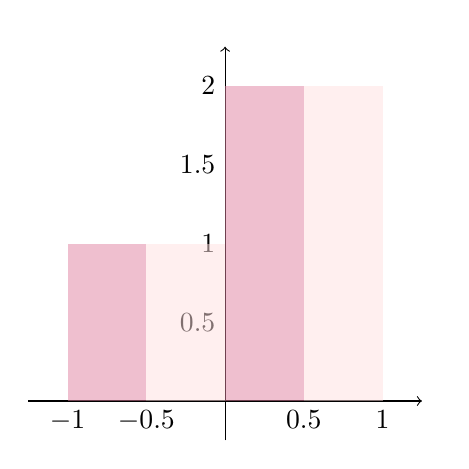
\begin{tikzpicture}[scale=2]

  % Zeichne das Koordinatensystem
  \draw[->] (-1.25,0) -- (1.25,0) node[right] {\(\)}; % x-Achse
  \draw[->] (0,-0.25) -- (0,2.25) node[above] {\(\)};  % y-Achse

  % Gitterlinien und Beschriftungen (im 0.5-Schritt)
  \foreach \x in {-1,-0.5,0.5,1} {
    \node[below] at (\x,0) {\(\x\)};
  }
  \foreach \y in {0.5,1,1.5,2} {
    \node[left] at (0,\y) {\(\y\)};
  }

  % Zeichne die eingefärbte Fläche (unter der Linie bis 0)
  \fill[purple!50,opacity=0.5] (-1,0) -- (-1,1) -- (-0.5,1) -- (-0.5,0) -- cycle; % Fläche x ∈ [-1, 0], y = 1
  \fill[pink!50,opacity=0.5] (-0.5,0) -- (-0.5,1) -- (0,1) -- (0,0) -- cycle; % Fläche x ∈ [0, 1], y = 2
  \fill[purple!50,opacity=0.5] (0,0) -- (0,2) -- (0.5,2) -- (0.5,0) -- cycle; % Fläche x ∈ [-1, 0], y = 1
  \fill[pink!50,opacity=0.5] (0.5,0) -- (0.5,2) -- (1,2) -- (1,0) -- cycle; % Fläche x ∈ [0, 1], y = 2

  % Zeichne den Graphen
  % \draw[thick,blue] (-1,1) -- (0,1); % Für x(-1,0), y = 1.0
  % \draw[thick,green] (0,2) -- (1,2); % Für x(0,1), y = 2.0

  % Zeichne die Linien von der x-Achse bis zur oberen Linie
  % \foreach \x in {-1,-0.75,-0.5,-0.25,0} {
  %   \draw[dotted] (\x,0) -- (\x,1); % Linien für x ∈ [-1, 0], y = 1
  % }
  % \foreach \x in {0,0.25,0.5,0.75,1} {
  %   \draw[dotted] (\x,0) -- (\x,2); % Linien für x ∈ [0, 1], y = 2
  % }

\end{tikzpicture}
\end{center}
\subsection{Maximum-Likelihood-Methode}
Seien $X_1,X_2,\dots,X_n$ unabhängige, auf $[0,\theta], \theta>0$, gleichverteilte Zufallsvariablen. Bestimmen Sie den Maximum-Likelihood-Schätzer $\theta_\ast$ für den unbekannten Parameter $\theta$. Ist der Schätzer erwartungstreu? Begründen Sie jeweils kurz.\\
\textit{Hinweis}: Beide Teile können ohne umfangreiche Rechnungen gelöst werden.\\\\
Gegeben:\\
$X_i \sim \mathbb{U}[0, \theta], \theta > 0$\\\\
Weil $X_i$ stetig gleichverteilt ist, hat $X_i$ die Dichte:\\\\
\[f_{X_i} (x)=\begin{cases}
    \frac{1}{\theta}, & \text{falls } 0 \leq x \leq \theta \\
    0, & \text{sonst}
\end{cases}\]
Somit können wir die \textit{Likelihood-Funktion} aufstellen:\\
$L(X_1, ..., X_n) = \prod\limits_{i = 1}^n f_x(X_i) = \left( \frac{1}{\theta} \right)^n \quad | \quad 0 \leq X_i \leq \theta$\\\\
Nun Maximieren wir mit $\underset{\theta}{arg\,\mathrm{max}}\quad L(X_1, ..., X_n)$:\\\\
- Die \textit{Likelyhood-Funktion} wird maximal, wenn $\theta$ am kleinsten ist (so klein wie möglich).\\
- $\theta$ muss indestens so groß sein wie der größte Wert aus $X_1, ..., X_n$\\\\
Somit ergibt sich:\\
\[f_{X_i} (x)=\begin{cases}
    \frac{1}{\theta}, & \theta \geq \max(X_1, ..., X_n) \\
    0, & \theta < \max(X_1, ..., X_n)
\end{cases}\]
- da so das kleinstmögliche $\theta = \max(X_1, ..., X_n)$ ist und $X_i$ stetig auf $[0, \theta]$ gleichverteilt sind, gilt: $\theta \geq X_i = \max(X_1, ..., X_n)$.\\
- ist erwartunstreu, wenn $\mathbb{E}(\max(X_1, ..., X_n)) = \theta$\\
$\Rightarrow \max(X_1, ..., X_n) < \theta$ und $\mathbb{E}(\max(X_1, ..., X_n)) < \theta$. Dies weist eine Ungleichheit auf, und der Schätzer $\theta_*$ welcher gleich $\max(X_1, ..., X_n)$, ist somit nicht erwartungstreu.
\\\\

\subsection{}
Die Zahl der Verkehrsunfälle in einer Stadt lag im letzen Jahr an zehn zufällig gewählten, regenfreien Tagen bei
\[4\quad 0\quad 6\quad 5\quad 2 \quad 1\quad 2\quad 0\quad 4\quad 3\]
Die Anzahl der Unfälle an einem regenfreien Tag sei poissonverteilt mit unbekanntem Parameter $\theta$. Wir suchen nun nach einem Schätzer $T$ für $\theta$ mit der A-priori  Information, dass T exponentialverteilt mit Parameter $\lambda = 2$ ist.\\\\
(a) Ermitteln Sie einen Schätzer für den Parameter $\theta$ für allgemeines (aber festes) $\lambda$ und unabhängige Beobachtungen $X_1,\dots, X_n$. Ist dieser konsistent oder erwartungstreu?\\\\
Gegeben sind:\\
Die gegebenen Werte sind Poissonverteilt (wobei $n = 10$), also $X_{1, ..., 10} \sim Poi(\theta)$\\
Die Formel zur Berechnung der Wahrscheinlichkeit eines einzelnen Ereignisses der Poissonverteilung ist: $\mathbb{P}(X_i = k) = \frac{\theta^k}{k!} \cdot e^{- \theta}$ wobei $\mathbb{E}(X_i) = \theta$\\
Aus der Aufgabe: $T \sim Exp(\lambda)$\\
Die Verteilungsfunktion F ist wie bereits bekannt, die Stammfunktion von f, der Dichte.\\\\
Der Schätzer $T$ ist als exponentielle Zufallsvariable definiert, daher muss eine \textit{Bayes-Schätzung} vorgenommen werden\\
Zunächst stellen wir die \textit{Likelihood-Funktion} auf:\\\\
$L((X1, ..., X_n), \theta) = \mathbb{P}(X_1, ..., X_n = X_n \,|\, T = \theta) = \prod\limits_{i = 1}^n \mathbb{P}(X_i = X_i \,|\, T = \theta) = \prod\limits_{i = 1}^n \frac{\theta^{X_i}}{X_i!}e^{- \theta}$\\\\
Nun definieren wir den \textit{MAP-Schätzer}\\\\
$\overline{\theta}_{MAP}(X_1, ..., X_n) = \underset{\theta}{arg\,\mathrm{max}}\,\, L((X_1, ..., X_n), \theta) f_T(\theta)$\\
Das gilt, weil \textit{T} stetig und $X_i$ diskret ist.\\\\
$\Rightarrow \overline{\theta}(X_1, ..., X_n) = \underset{\theta}{arg\,\mathrm{max}}\,\, \left( \prod\limits_{i = 1}^n \frac{\theta^{X_i}}{X_i!}e^{- \theta} \right) \ \lambda e^{- \lambda \theta}$\\
\hspace*{2.57cm}$= \underset{\theta}{arg\,\mathrm{max}}\,\, \ln\left(\left( \prod\limits_{i = 1}^n \frac{\theta^{X_i}}{X_i!}e^{- \theta} \right) \cdot \lambda e^{- \lambda \theta} \right)$\\
\hspace*{2.57cm}$= \underset{\theta}{arg\,\mathrm{max}}\,\, \left(\sum\limits_{i = 1}^n \ln\left( \frac{\theta^{X_i}}{X_i!}e^{- \theta} \right)\right) + \ln\left(\lambda \right) - \lambda \theta$\\
\hspace*{2.57cm}$= \underset{\theta}{arg\,\mathrm{max}}\,\, \left(\sum\limits_{i = 1}^n \ln\left( \frac{\theta^{X_i}}{X_i!}\right) - \theta \right) + \ln\left(\lambda \right) - \lambda \theta$\\
\hspace*{2.57cm}$= \underset{\theta}{arg\,\mathrm{max}}\,\, \left(\sum\limits_{i = 1}^n X_i \cdot \ln\left( \theta\right) - \ln\left( X_i! \right) - \theta \right) + \ln\left(\lambda \right) - \lambda \theta$\\\\
Nun Leiten wir den Term nach $\theta$ ab und setzen  ihn gleich 0 um das Extrema und mögliches Maximum zu finden:\\\\
$\Rightarrow \frac{d \log(\lambda)}{d \theta} = \left( \sum\limits_{i = 1}^n \frac{X_i}{\theta} - 1 \right) - \lambda \overset{!}{=} 0$\\
\hspace*{1.27cm}$\Leftrightarrow \frac{1}{\theta} \left(\sum\limits_{i = 1}^n X_i \right) - n - 1 \overset{!}{=} 0$\\
\hspace*{3.3cm}$\Leftrightarrow \sum\limits_{i = 1}^n X_i = \theta (n + \theta)$\\
\hspace*{3.3cm}$\Leftrightarrow \theta_{MAP} = \frac{1}{n + \theta} \sum\limits_{i = 1}^n X_i$\\\\
Nun leiten wir die erste Ableitung erneut ab, um herauszufinden, ob das gefundene Extremum ein Minimum oder Maximum ist.\\\\
$\Rightarrow \frac{d^2\log(\lambda)}{d^2 \theta} = - \frac{1}{\theta^2} \sum\limits_{i = 1}^n X_i$.\\\\
$\theta^2$ muss größer oder gleich 0 sein für alle $\theta \in \Theta$, $- \frac{1}{\theta^2} < 0$ und somit ist der gesamte Term kleiner als 0. Damit ist bewiesen, dass das gefundene \textit{Extremum} ein \textit{Maximum} ist.\\\\
Damit ist dann gezeigt, dass die allgemeine \textit{MAP-Schätzung} $\theta_{MAP} = \frac{1}{n + \delta} \sum\limits_{i = 1}^n X_i$\\\\
Nun müssen wir noch zeigen, ob der \textit{Schätzer} konsistent und erwartungstreu ist:\\\\
\textit{Erwartungstreue: Gilt, wenn} $\mathbb{E}(\theta_{MAP}) = \theta$\\\\
$\mathbb{E}(\theta_{MAP}) = \mathbb{E}\left( \frac{1}{n + \lambda} \sum\limits_{i = 1}^n X_i \right) = \frac{1}{n + \lambda} \cdot \sum\limits_{i = 1}^n \mathbb{E}\left( X_i \right) = \frac{1}{n + \lambda} \ cdot \sum\limits_{i = 1}^n \theta = \frac{n \theta}{n + \lambda} \neq \lambda \, | \lambda > 0$\\
$\Rightarrow \theta_{MAP}$ Ist nicht erwartungstreu\\\\
\textit{Konsistenz: Gilt, wenn} $\lim\limits_{n \to \infty} \theta_{MAP} = \theta$\\\\
$\lim\limits_{n \to \infty} \theta_{MAP} = \lim\limits_{n \to \infty} \frac{1}{n + \lambda} \sum\limits_{i = 1}^n X_i = \lim\limits_{n \to \infty} \frac{1}{n(1 + \frac{\lambda}{n})} \sum\limits_{i = 1}^n X_i = \lim\limits_{n \to \infty} \frac{1}{1 + \frac{\lambda}{n}} \cdot \lim\limits_{n \to \infty} \frac{1}{n} \sum\limits_{i = 1}^n X_i = \lim\limits_{n \to \infty} \frac{1}{1 + \frac{\lambda}{n}} \cdot \theta = 1 \cdot \theta$\\
$\Rightarrow$ Somit ist $\theta_{MAP}$ konsistent.
\\\\
(b) Schätzen Sie $\lambda$ aus den obigen Daten.\\\\
Gegeben sind:\\
- $\lambda = 2$\\
- $n = 10$
- $\theta_{MAC} = \frac{1}{n + \lambda} \sum\limits_{i = 1}^n X_i$\\
$\Rightarrow \theta = \frac{1}{10 + 2} (4 + 0 + 6 + 9 + 2 + 1 + 0 + 4 + 3) = \frac{9}{4}$\\\\
(c) Schätzen Sie damit den Anteil der regenfreien Tage, an denen im letzten Jahr zwei oder weniger Verkehrsunfälle passierten.\\\\
Gesucht ist $\mathbb{P}(X_i \leq 2) = F_{X_i}(2) = \mathbb{P}(X_i = 0) + \mathbb{P})(X_i = 1) + \mathbb{P}(X_i = 2)$\\
$= \frac{\left( \frac{9}{4} \right)^0}{0!} \cdot e^{- \frac{9}{4}} + \frac{\left( \frac{9}{4} \right)^1}{1!} \cdot e^{- \frac{9}{4}} + \frac{\left( \frac{9}{4} \right)^2}{2!} \cdot e^{- \frac{9}{4}} \approx 0.609$\\\\
Somit ist der Anteil an regenfreien Tagen mit höchstens zwei Verkehrsunfällen im letzten Jahr ist circa 60.9\%. 

\subsection{}
Die folgende Tabelle zeigt die Anzahl der Tage mit Schneefall und die Anzahl der Zugausfälle bei der S-Bahn-Linie 85 in den Monaten eines Winters.\\\\
\begin{tabular}{l|c|c|c}
    Monat & Dezember & Januar & Februar \\
    \hline
    Anzahl Tage mit Schneefall & 3 & 5 & 4 \\
    \hline
    Anzahl Zugausfälle bei der S85 & 17 & 32 & 23\\
\end{tabular}\\\\
Von Interesse ist die Anzahl der Zugausfälle in Abhängigkeit mit der Anzahl der Tage mit Schneefall. Bestimmen Sie die Regressionsgerade.\\\\
Wir bestimmen $X$ als Tage mit Schneefall und $Y$ als Zugausfälle mit $X(\Omega)=\{3,5,4\}$ und $Y(\Omega)=\{17, 32, 23\}$.\\\\
empirisches Mittel:\\
\(\mu_n = \frac{1}{n} \sum\limits^n_{i=1} x_i\\
\mu_X=\frac{1}{3}(3+5+4)=4\\
\mu_Y=\frac{1}{3}(17+32+23)=24\)\\\\
empirische Standardabweichung:\\
\(\sigma^2_n= \frac{1}{n-1}\sum\limits^n_{i=1}(x_i-\mu)^2\)\\
\(\sigma_X^2=\frac{1}{3-1}\left((3-4)^2+(5-4)^2+(4-4)^2\right)=\frac{1}{2}(1+1+0)=1\)\\
\(\sigma^2_Y=\frac{1}{3-1}\left((17-24)^2+(32-24)^2+(23-24)^2\right)=\frac{1}{2}(49+64+1)=\frac{114}{2}=57\)\\\\
empirische Kovarianz:\\
\(c_{XY}:= \frac{1}{n-1}\sum\limits^n_{i=1}(x_i-\mu_X)(y_i-\mu_Y)\)\\
\(c_{XY} = \frac{1}{3-1}\left((3-1)(17-24)+(5-4)(32-24)+(4-4)(23-24)\right)=\frac{1}{2}(7+8+0)=\frac{15}{2}=7.5\)\\\\
lineare Regression:\\
\(y=ax+b\quad a=\frac{c_{XY}}{\sigma_X}\quad b=\mu_Y\cdot a \cdot \mu_X\)\\
\(a=\frac{7,5}{1}=7.5\quad b=24\cdot 7.5 \cdot 4=-6\)\\
\(y=7.5x-6\)
\end{document}
